				\chapter{Review of Literature }
				\section{Summary of the investigation in the published papers}
				
				\begin{itemize}
				\item \textbf{Computer Algorithms for Plagiarism Detection}
				
				Described the various levels of plagiarism and the different metrics(approaches) like Halstead metric, ACCUSE metric, FORTRAN programs, etc. This paper also compared different algorithms based on the software metrics used. The different levels of plagiarism defined in this paper will form the foundation of our project and we’ll be looking to detect plagiarism based on these levels.
				
				
				
				\begin{figure}[h]	
				\centering			
					\includegraphics[width=0.8\textwidth]{LevelDiag}
	  				\label{fig:Level1}
	  				\caption{Spectrum of Plagiarism}
					\end{figure}
				
				
				\pagebreak
				
				\item \textbf{A Comparison of Similarity Techniques for Detecting Source Code Plagiarism}
				
				This paper outlines different modern approaches to software similarity measurement. Algorithms like Levenshtein edit distance, Tree edit distance and graph edit distance were discussed. Knowledge of different approaches was gained and this will help us choose our approach.
				
				\item  \textbf{An Approach to Source-Code Plagiarism Detection and Investigation Using Latent Semantic Analysis}
				
				Latent Semantic Analysis, a statistical approach to detecting similarity is analysed in-depth in this paper. This paper also has an exhaustive description of what constitutes Plagiarism which includes surveys and research papers. Deeper understanding of Plagiarism was made possible by this research paper.
				
				\item  \textbf{Plagiarism Detection in Java Code}
				
				This thesis gives a step-by-step procedure on how to detect plagiarism in java source code using the Levenshtein Edit distance algorithm. It uses different normalization techniques and demonstrates these techniques using examples. Normalization techniques shown inn this thesis will be used in our project.
				
				\item \textbf{Source Code Plagiarism Detection ‘SCPDet’: A Review}
				
				In this paper author describes the real meaning of source code plagiarism and  then described the different source code plagiarism detection tools and compared its function, characteristics and technique. In the last phase, authors discussed the different research papers and compared in tabular form with its technique, method, characteristics, functionality and its result.
				
				\end{itemize} 
				
\newpage
				\section{Comparison between the tools / methods / algorithms}\begin{table}[!htbp]
				  \centering
				  \caption{Compression of four source code detection tools with its characteristics, function and technique}
				  \label{tab:table1}
				  \begin{tabular}{|p{3cm}|p{3cm}|p{3cm}|p{3cm}|p{3cm}|}
				\hline 
				Tools & JPlag & SIM & MOSS & Plaggie \\ \hline
				
				Open Source Tools/Paid & NO & YES & NO & YES \\ \hline
				Local/online tool & Web & Local & Web & Local  \\ \hline
				Code Submit/File & Submit Code & Submit File & Submit
				Code & Submit Code  \\ \hline
				Lang. Support & 6 & 5 & 23 & 1 \\ \hline
				Expandability & No & Yes & No & No \\ \hline
				Founded in Year & 1996 & 1989 & 1994 & 2002 \\ \hline
				Founded By  & Guido Malpohl & Dick Grune & Aiken & Ahtiaine \\ \hline
				
				Technique & Greedy String Tiling and Optimization and Tokenization & Flax lexical analyzer & Winnowing technique & Greedy String Tiling and Tokenization \\ \hline	\end{tabular}
				
				\vspace{40 mm}
				
				  \centering
				  \caption{Comparison between different metrics : Structural Metrics and Similarity Metrics}
				  \label{tab:table2}
				  \begin{tabular}{|p{6cm}|p{6cm}|}
				\hline 
				Structural metrics & Similarity metrics  \\ \hline
				
				Structural metrics – no. of variables, no. of keywords, no. of loops, no. of comment lines & Similarity metrics – no. of characters per line, no of code lines, no. of blank lines \\ \hline
				
				Structural metrics represent information about programming constructs and elements used in the code. & Similarity metrics are indicative of the style used in programming and are effective in detecting plagiarism. \\ \hline	
				
				
				Lots of rudimentary plagiarism detection algorithms like Halstead use only structural metrics and are ineffective for larger programs. &  Modern approaches include algorithms that use a combination of structural and similarity metrics to detect plagiarism and are highly effective. \\ \hline 
				
				\end{tabular}
						
				
				
				\end{table}  
				
				
				
				
	\pagebreak
				
				\section{Algorithms}
				
				\begin{itemize}
				
				\item \textbf{Level 0 Plagiarism Pseudo-Code}
					\begin{figure}[h]
					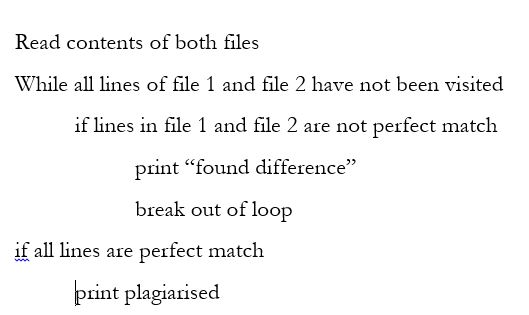
\includegraphics[width=0.8\textwidth]{Level0Alg}
	  				\label{fig:Level0}
	  				\end{figure}
	  				
				
				\item \textbf{Level 1 Plagisrism Pseudo-Code}
					\begin{figure}[!h]				
					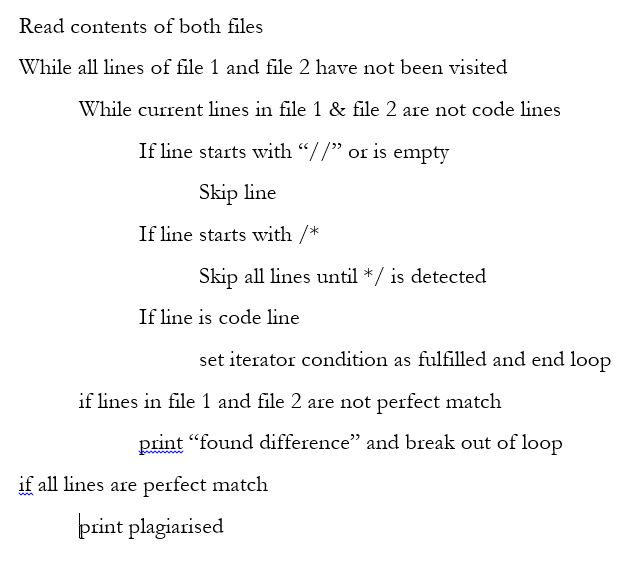
\includegraphics[width=0.8\textwidth]{Level1Alg}
	  				\label{fig:Level1}
					\end{figure}
					
				\pagebreak				
	
				\item \textbf{Level 3 Plagisrism Pseudo-Code}\\
					\begin{figure}[h]				
					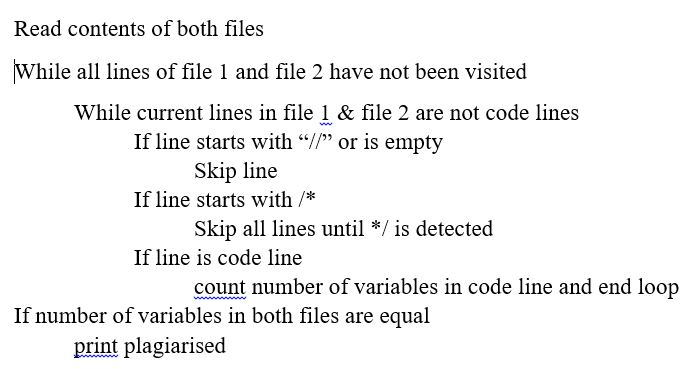
\includegraphics[width=0.8\textwidth]{Level3Alg}
	  				\label{fig:Level3}	
	  				\end{figure}		
				
				\end{itemize} 
				
				
				
				
				
				
				
				
				
				
				
				
				
				
				
				
				
				
				